\documentclass{article}
\usepackage[T1]{fontenc}
\usepackage[utf8]{inputenc}
\usepackage{lmodern}
\usepackage[ngerman]{babel}
\usepackage{amsmath, amssymb}
\usepackage{array}
\usepackage{hyperref}
\usepackage{graphicx}
\usepackage{tikz, tikzsymbols}
\usepackage{xcolor}
\usepackage{algorithm2e}

\usetikzlibrary{arrows,automata,fit}
\setlength\parindent{0pt}

\begin{document}

\begin{center}
  \Large{Informatik \rotatebox[origin=c]{180}{D}\raisebox{0.05em}{:} Übungsblatt 10}

  \large{Sebastian Höffner, Andrea Suckro}
\end{center}



\section*{Aufgabe 10.1}
\subsection*{a)}
Der Algorithmus $\mathcal{A}$ berechnet $3^{\left(3^x\right)}$.


\subsection*{b)}
Das uniforme Kostenmaß berücksichtigt nicht, dass die Werte für $y$ sehr schnell sehr groß werden und die Multiplikation rasch über 32 oder 64 bit Zahlen hinausreicht.
Insbesondere ist dank $\log_3(\log_3(18.446.744.073.709.551.615)) \approx 3,366$ ab einer Eingabe von $x > 3,366$ ein Overflow gegeben.

Im uniformen Kostenmaß wäre die Laufzeit immer $\mathcal{O}(n)$, da aber die Funktion $3^{\left(3^x\right)}$ exponentiell wächst, müssen die Multiplikationen später länger dauern.


\subsection*{c)}
Wir definieren:
\begin{itemize}
	\item $\mathcal{K}(x)$: Kosten bei Eingabe $x$
	\item $y_i$: Wert von $y$ vor $i$-tem Schleifeneintritt
\end{itemize}

Dann sind die Kosten
\begin{align*}
\mathcal{K}(x) &= \sum\limits_{i=1}^x 3 \left(log y_i\right)^2
\end{align*}
 


\section*{Aufgabe 10.2}

\subsection*{a)}
\begin{align*}
\left(\max\limits_{x\in\mathbb{R}^n}\left\{c^Tx\middle|Ax\leq b\right\}, k\right), \exists x: \left(c^Tx\geq k, Ax \leq b\right)
\end{align*}
Das heißt, das Entscheidungsproblem ist: "`Gibt es ein $x$, sodass $c^Tx \geq k$ mit $Ax \leq b$ erfüllt ist?"'
Oder anders gesagt, der Algorithmus $\mathcal{A}$ aus Aufgabe b) gibt \texttt{true} zurück, wenn $c^Tx$ größer oder gleich dem Inputparameter $k_i$ ist, sonst \texttt{false}.

\subsection*{b)}
Wir können dank der Einschränkungen von $c$ und $x$ auf "`binäre"' Vektoren annehmen, dass $0 \leq c^Tx \leq n$ ist.
Das heißt, wir müssen lediglich für alle Zahlen $0\dots n$ das Entscheidungsproblem prüfen, um das Optimierungsproblem zu lösen. 

Naiv könnten wir dazu einfach alle Zahlen testen (Siehe Algorithmus \ref{alg:2naiv}). Dieser Algorithmus hat allerdings dann eine Laufzeit von $\mathcal{O}\left(t_\mathcal{A}\left(m,n\right)n\right)$.

Besser ist eine Binäre Suche. Diesen Algorithmus kennen wir noch aus Informatik A bzw. aus dem Alltag ("`Ich denke mir eine Zahl von 1 bis 100 und sage dir zu deinen Tipps, ob sie größer oder kleiner ist."'). Der Algorithmus \ref{alg:2logn} hat die gewünschte Laufzeit von $\mathcal{O}\left(t_\mathcal{A}\left(m,n\right)\log{n}\right)$. (Der geneigte Leser findet eine Implementation in Java mit Tests \href{http://uni.sebastian-hoeffner.de/DInf/DInf14102b.java}{hier}).

\begin{algorithm}
\DontPrintSemicolon
max = -$\infty$\;
\For{i = $0\dots n$}{
  \eIf{$\mathcal{A}(i)$}{
    max = i\;
  }{
    \Return{max}\;
  }
}
\Return{max}\;
\label{alg:2naiv}
\caption{Naiver Algorithmus für das Optimierungsproblem}
\end{algorithm}

\begin{algorithm}
  \DontPrintSemicolon
  \KwIn{$n$}
  \KwOut{$\max\limits_{x\in\mathbb{R}^n}\left\{c^Tx\middle|Ax\leq b\right\}$}
  \tcp{Initializations}
  array $ks$ := $\left\{0, \dots, n\right\}$\;
  $left$     := 0\;
  $right$    := n - 1\;
  $middle$   := ($left$ + $right$) / 2\;
  \While{$left < right$}{
    \eIf{$\mathcal{A}\left(ks\left[middle\right]\right)$}{
      \tcp{adjust boundaries}
      $left$   := $middle$ + 1\;
      $middle$ := ($left$ + $right$) / 2\;
      \tcp{decision problem is $\geq$, so we check another value}
      \If{$\neg\mathcal{A}\left(ks\left[left\right]\right)$}{
        \Return{$left - 1 \geq 0? ks\left[left - 1\right] : -1$}
      }
    }{
      \tcp{adjust boundaries}
      $right$  := $middle$ - 1\;
      $middle$ := ($left$ + $right$) / 2\;
    }
  }
  \tcp{left <= right -> middle element is optimum, or not optimizable}
  \If{$\mathcal{A}\left(ks\left[middle\right]\right)$}{
    \Return{$ks\left[middle\right]$}
  }
  \Return{-1}
  \label{alg:2logn}
  \caption{Möglicher Algorithmus in $\mathcal{O}\left(t_\mathcal{A}\left(m,n\right)\log{n}\right)$}
\end{algorithm}



\section*{Aufgabe 10.3}
\subsection*{a)}
Man kann die Erfüllbarkeit in linearer Zeit (linear in Relation zur Anzahl Literale) testen, indem man für alle einzelnen Konjunktionsterme prüft, ob sie einen Widerspruch beinhalten -- sobald ein Term keinen Widerspruch enthält, können wir abbrechen. Das liegt daran, dass nur im Fall, dass alle Terme Widersprüche enthalten, eine DNF \texttt{false} sein kann.

\subsection*{b)}
Der Beweis geht davon aus, dass die Umwandlung in polynomieller Zeit geschieht. Doch eine aus einer KNF erzeugte DNF hat $2^n$ Terme die Umwandlung muss also exponentiell sein:

\begin{align*}
KNF &\Rightarrow DNF \\
\bigwedge\limits_i^n \left(A_i \vee B_i\right) &\Rightarrow \bigvee\limits_{X\in\left\{A,B\right\}^n} \left(X_1 \wedge \dots \wedge X_n\right)
\end{align*}



\section*{Aufgabe 10.4}
Es gibt 3 Stunden und 4 Verdächtige, also folgende Variablen:
\begin{align*}
\begin{array}{l|lll}
\text{Tyrions Lebensstatus} & y_1 & y_2 & y_3 \\
\hline
\text{Verdächtiger $v$ in Tyrions} & x_{Sansa,1} & x_{Sansa,2} & x_{Sansa,3} \\ 
\text{Gemächern zum Zeitpunkt $t$} & x_{Shae,1} & x_{Shae,2} & x_{Shae,3} \\
x_{v,t}                            & x_{Stannis,1} & x_{Stannis,2} & x_{Stannis,3} \\
                                   & x_{Sandor,1} & x_{Sandor,2} & x_{Sandor,3} \\
\end{array}
\end{align*}

Die einzelnen Formeln für die Fakten (1)-(7) sind (aus Platzgründen etwas umgeordnet):

\smallskip

\textbf{(1): }Stannis und Sansa sprechen entweder gemeinsam in Tyrions Gemächern oder gemeinsam außerhalb.
\begin{align*}
\mathcal{F}_{1}=(x_{Sansa,1} \wedge x_{Stannis,1}) \vee (\neg x_{Sansa,1} \wedge \neg x_{Stannis,1})
\end{align*}

\textbf{(5): }Sansa und Shae sind in Stunde 2 am selben Ort.
\begin{align*}
\mathcal{F}_5 = \left( \neg x_{Sansa,2} \wedge \neg x_{Shae,2} \right) \vee \left( x_{Sansa,2} \wedge x_{Shae,2} \right)
\end{align*}

\textbf{(6): }Shae ist in der zweiten Stunde in Tyrions Gemächern.
\begin{align*}
\mathcal{F}_6 = x_{Shae,2}
\end{align*}

\textbf{(4): }Sansa war in Stunde 1 und 2 am selben Ort und in Stunde 3 nicht in Tyrions Gemächern.
\begin{align*}
\mathcal{F}_4 = \left( \left( \neg x_{Sansa,1} \wedge \neg x_{Sansa,2} \right) \vee \left( x_{Sansa,1} \wedge x_{Sansa,2} \right) \right) \wedge \neg x_{Sansa,3}
\end{align*}

\textbf{(2): }Alle Kombinationen aus einem oder zwei Verdächtigen zu jeweils den Zeitpunkten t sind gültig.
\begin{align*}
\mathcal{F}_{2}=
\bigwedge\limits_{t=1}^{3} \left(\right. & \\
\text{\small\textit{Ein Verdächtiger:}} \\
                                         & \left(      x_{Sansa,t} \wedge \neg x_{Shae,t} \wedge \neg x_{Stannis,t} \wedge \neg x_{Sandor,t} \right)\\
                                    \vee & \left( \neg x_{Sansa,t} \wedge      x_{Shae,t} \wedge \neg x_{Stannis,t} \wedge \neg x_{Sandor,t} \right)\\
                                    \vee & \left( \neg x_{Sansa,t} \wedge \neg x_{Shae,t} \wedge      x_{Stannis,t} \wedge \neg x_{Sandor,t} \right)\\
                                    \vee & \left( \neg x_{Sansa,t} \wedge \neg x_{Shae,t} \wedge \neg x_{Stannis,t} \wedge      x_{Sandor,t} \right)\\
\text{\small\textit{Zwei Verdächtige:}} \\
                                    \vee & \left(      x_{Sansa,t} \wedge      x_{Shae,t} \wedge \neg x_{Stannis,t} \wedge \neg x_{Sandor,t} \right)\\
                                    \vee & \left(      x_{Sansa,t} \wedge \neg x_{Shae,t} \wedge      x_{Stannis,t} \wedge \neg x_{Sandor,t} \right)\\
                                    \vee & \left(      x_{Sansa,t} \wedge \neg x_{Shae,t} \wedge \neg x_{Stannis,t} \wedge      x_{Sandor,t} \right)\\
                                    \vee & \left( \neg x_{Sansa,t} \wedge      x_{Shae,t} \wedge      x_{Stannis,t} \wedge \neg x_{Sandor,t} \right)\\
                                    \vee & \left( \neg x_{Sansa,t} \wedge      x_{Shae,t} \wedge \neg x_{Stannis,t} \wedge      x_{Sandor,t} \right)\\
                                    \vee & \left( \neg x_{Sansa,t} \wedge \neg x_{Shae,t} \wedge      x_{Stannis,t} \wedge      x_{Sandor,t} \right)\\ 
                                         & \left.\right)
\end{align*}

\textbf{(3): }Für Stannis und Shae darf je nur ein t erfüllt sein:
\begin{align*}
\mathcal{F}_3 = \left(\right. & \left(x_{Shae,1} \wedge \neg x_{Shae,2} \wedge \neg x_{Shae,3} \right) \\ 
                         \vee & \left(\neg x_{Shae,1} \wedge x_{Shae,2} \wedge \neg x_{Shae,3} \right) \\ 
                         \vee & \left(\neg x_{Shae,1} \wedge \neg x_{Shae,2} \wedge x_{Shae,3} \right) \left.\right)\\
                       \wedge & \\
                \left(\right. & \left(x_{Stannis,1} \wedge \neg x_{Stannis,2} \wedge \neg x_{Stannis,3} \right) \\ 
                         \vee & \left(\neg x_{Stannis,1} \wedge x_{Stannis,2} \wedge \neg x_{Stannis,3} \right) \\ 
                         \vee & \left(\neg x_{Stannis,1} \wedge \neg x_{Stannis,2} \wedge x_{Stannis,3} \right) \left.\right)
\end{align*}

\textbf{(7): }Wenn Shae nicht mehr in Tyrions Gemächern ist, ist er tot.
\begin{align*}
\mathcal{F}_7 = & \left(x_{Shae,1} \wedge y_1 \wedge x_{Shae,2} \wedge y_2 \wedge x_{Shae,3} \wedge y_3 \right) \\
           \vee & \left(x_{Shae,1} \wedge y_1 \wedge x_{Shae,2} \wedge y_2 \wedge \neg x_{Shae,3} \wedge \neg y_3 \right) \\
           \vee & \left(x_{Shae,1} \wedge y_1 \wedge \neg x_{Shae,2} \wedge \neg y_2 \wedge \neg x_{Shae,3} \wedge \neg y_3 \right) \\
           \vee & \left(\neg x_{Shae,1} \wedge \neg y_1 \wedge \neg x_{Shae,2} \wedge \neg y_2 \wedge \neg x_{Shae,3} \wedge \neg y_3 \right)
\end{align*}

\textbf{Zusatz: }Tote Menschen bleiben tot.
\begin{align*}
\mathcal{F}_8 = \left(y_1 \wedge y_2 \wedge \neg y_3\right) \vee \left(y_1 \wedge \neg y_2 \wedge \neg y_3\right) \vee \left(\neg y_1 \wedge \neg y_2 \wedge \neg y_3\right)
\end{align*}


Alle Formeln müssen gleichzeitig gültig sein, also $\mathcal{F}_1 \wedge \mathcal{F}_2 \wedge \mathcal{F}_3 \wedge \mathcal{F}_4 \wedge \mathcal{F}_5 \wedge \mathcal{F}_6 \wedge \mathcal{F}_7 \wedge \mathcal{F}_8$.

Zum Lösen können wir mit (6) beginnen und $x_{Shae,2} = $ \texttt{true} setzen.

Nach (5) muss nun $x_{Sansa,2} = $ \texttt{true} sein, was nach (4) ebenfalls zu $x_{Sansa,1} = $ \texttt{true} führt. Ebenfalls nach (4) ist klar, dass $x_{Sansa,3} = $ \texttt{false} ist. Nach (1) folgt nun, dass Stannis mit Sansa in Tyrions Gemächern war ($x_{Stannis,1} = $ \texttt{true}). 

Nach (2) kann geschlussfolgert werden, dass $x_{Shae,1} = $ \texttt{false}, $x_{Sandor,1} = $ \texttt{false},  $x_{Stannis,2} = $ \texttt{false} und $x_{Sandor,2} = $ \texttt{false}. Weiterhin führen die bisherigen Beobachtungen zu der Erkenntnis, dass Stannis und Shae nach (3) in Stunde 3 nicht in Tyrions Gemächern waren ($x_{Shae,3} = $ \texttt{false}, $x_{Stannis,3} = $ \texttt{false}).

Automatisch folgt nach (7), dass Tyrion in Stunde 3 gestorben sein muss ($y_3= $\\\texttt{false}, $y_2= $ \texttt{true} und $y_1= $ \texttt{true}).

Da Tyrion in Stunde 3 stirbt, für drei Verdächtige jedoch ausgeschlossen wurde, dass sie in dieser Stunde in seinen Gemächern waren, bleibt nur noch die Möglichkeit, dass Sandor in der dritten Stunde in Tyrions Gemächern war und Tyrion dort umbrachte ($x_{Sandor,3} = $ \texttt{true}).

\begin{align*}
\begin{array}{l|lll}
\text{Tyrions Lebensstatus}        & y_1 = t & y_2 = t & y_3 = f \\
\hline
\text{Verdächtiger $v$ in}   & x_{Sansa,1}   = t & x_{Sansa,2}   = t & x_{Sansa,3}   = f \\ 
\text{Tyrions Gemächern zum} & x_{Shae,1}    = f & x_{Shae,2}    = t & x_{Shae,3}    = f \\
\text{Zeitpunkt $t$}         & x_{Stannis,1} = t & x_{Stannis,2} = f & x_{Stannis,3} = f \\
x_{v,t}                      & x_{Sandor,1}  = f & x_{Sandor,2}  = f & x_{Sandor,3}  = t \\
\end{array}
\end{align*}
Der Mörder war also wahrscheinlich \emph{Sandor Clegane} in der \emph{dritten Stunde}. (Unter den Annahmen, dass Tyrion keinen Selbstmord beging bzw. Sansa und Shae ihn nicht beim Verlassen des Raumes am Ende der zweiten Stunde erdolchten, was ebenfalls zu einem Tod in Stunde drei hätte führen können -- schließlich hatte Tyrion noch Zeit, den Hinweis zu schreiben.)



\section*{Aufgabe 10.5}
\begin{figure}
  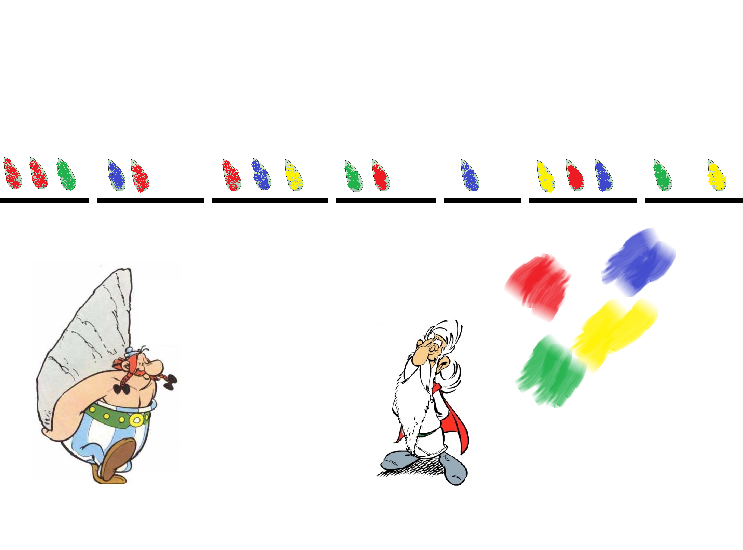
\includegraphics[width=\columnwidth]{hinkelsteine.png}
  \caption{Veranschaulichung der Aufgabe 10.5}
  \label{fig:obelix}
\end{figure}

\subsection*{a)}
Die Anzahl Hinkelsteine pro Haufen ist auf drei begrenzt. Dadurch ergeben sich folgende mögliche Farbkombinationen $K_1,\dots,K_6$ mit jeweils den Farben $a, b, c$:
\begin{align*}
K_1 &= \left\{ a, b, c \right\} \\
K_2 &= \left\{ a, a, b \right\} \\
K_3 &= \left\{ a, a, a \right\} \\
K_4 &= \left\{ a, b \right\} \\
K_5 &= \left\{ a, a \right\} \\
K_6 &= \left\{ a \right\} 
\end{align*}

Die Bedingungen für das \textsc{Sat}problem können nun für jeden Haufentypen bestimmt werden. Im Allgemeinen bedeuten sie: Falls eine Farbe $f_1$ in die Menge der schönen Farben $F_{schön}$ gewählt wurde und es nur einen Stein der Farbe $f_1$ auf dem Haufen $H_i$ gibt, so muss eine weitere Farbe $f_2$ aus dem Haufen $S_i$ in $F_{schön}$ gewählt werden, um das \textsc{Sat}problem zu erfüllen. Einige Klauseln sind dabei automatisch erfüllt, z.B. $K_3$.

In der Musterlösung wurden uns Implikationen gegeben, diese können jedoch durch $a \rightarrow b = \neg a \vee b$ aufgelöst werden. Die aufgelösten Formeln sind hier ebenfalls angegeben.

\begin{align*}
K_1 &= \left\{ a, b, c \right\} & \Rightarrow &&& \left(a \rightarrow (b \vee c) \right) \wedge \left(b \rightarrow (a \vee c) \right) \wedge \left(c \rightarrow (a \vee b) \right) \\
    &                           &             &&& \left(\neg a \vee b \vee c \right) \wedge \left(a \vee \neg b \vee c \right) \wedge \left(a \vee b \vee \neg c \right) \\
K_2 &= \left\{ a, a, b \right\} & \Rightarrow &&& b \rightarrow a \\
    &                           &             &&& \neg b \vee a \\
K_3 &= \left\{ a, a, a \right\} & \Rightarrow &&& a \vee \neg a \equiv \text{\texttt{true}} \\
K_4 &= \left\{ a, b \right\}    & \Rightarrow &&& \left( a \rightarrow b \right) \wedge \left( b \rightarrow a \right) \\
    &                           &             &&& \left( \neg a \vee b \right) \wedge \left( a \vee \neg b \right) \\
K_5 &= \left\{ a, a \right\}    & \Rightarrow &&& a \vee \neg a \equiv \text{\texttt{true}} \\
K_6 &= \left\{ a \right\}       & \Rightarrow &&& \neg a 
\end{align*}

Diese Klauseln werden nun für jeden Haufen $H$ ausgewählt und mit den entsprechenden Farben aufgefüllt. Für das Beispiel in Abbildung \ref{fig:obelix} sähe das wie folgt aus ($gr$ = grün gewählt, $ge$ = gelb gewählt, $b$ = blau, $r$ = rot).
\begin{align*}
       &\left(\neg gr \vee r \right) \\
\wedge &\left( \left( \neg b \vee r \right) \wedge \left( b \vee \neg r \right) \right) \\
\wedge &\left( \left(\neg r \vee b \vee ge \right) \wedge \left(r \vee \neg b \vee ge \right) \wedge \left(r \vee b \vee \neg ge \right) \right) \\
\wedge &\left( \left( \neg gr \vee r \right) \wedge \left( gr \vee \neg r \right) \right) \\
\wedge &\left( \neg b \right) \\
\wedge &\left( \left(\neg ge \vee r \vee b \right) \wedge \left(ge \vee \neg r \vee b \right) \wedge \left(ge \vee r \vee \neg b \right) \right) \\
\wedge &\left( \left( \neg gr \vee ge \right) \wedge \left( gr \vee \neg ge \right) \right) \\
\end{align*}

Vergessen dürfen wir aber nicht den wichtigsten Constraint: Dass die Farbe $l$ bereits gewählt wurde. Wir ketten dies an die Formel zuvor an ($\wedge l$). Nehmen wir für unser Beispiel an, gelb sei die Farbe $l$.
\begin{align*}
       &\left(\neg gr \vee r \right) \\
\wedge &\left( \left( \neg b \vee r \right) \wedge \left( b \vee \neg r \right) \right) \\
\wedge &\left( \left(\neg r \vee b \vee ge \right) \wedge \left(r \vee \neg b \vee ge \right) \wedge \left(r \vee b \vee \neg ge \right) \right) \\
\wedge &\left( \left( \neg gr \vee r \right) \wedge \left( gr \vee \neg r \right) \right) \\
\wedge &\left( \neg b \right) \\
\wedge &\left( \left(\neg ge \vee r \vee b \right) \wedge \left(ge \vee \neg r \vee b \right) \wedge \left(ge \vee r \vee \neg b \right) \right) \\
\wedge &\left( \left( \neg gr \vee ge \right) \wedge \left( gr \vee \neg ge \right) \right) \\
\wedge & ge
\end{align*}


\subsection*{b)}
Dieses Problem kann einfacher gelöst werden als gewöhnliche \textsc{Sat}probleme.
\begin{algorithm}[h]
\While{$\exists$ Haufen mit genau einem Hinkelstein \tcp{$\mathcal{O}(n)$}}{
  H = alle Haufen mit genau einem Hinkelstein \tcp{$\mathcal{O}(n)$}
  X = alle Farben aus H \tcp{$\mathcal{O}(n+m)$}
  \If{$l \in X$ \tcp{$\mathcal{O}(m)$}}{\Return{false}} 
  lösche alle Hinkelsteine der Farben X \tcp{$\mathcal{O}(nm)$}
}
\Return{true} \tcp{$\mathcal{O}(1)$}
\end{algorithm}
Der Algorithmus hat eine Gesamtlaufzeit von $\mathcal{O}(n) \cdot \mathcal{O}(nm) = \mathcal{O}(n^2m)$.



\section*{Aufgabe 10.6}
Für $\mathcal{X}=$\textsc{Sat} fixiert man die erste Variable und prüft, ob $\mathcal{A_X}$ \texttt{true} oder \texttt{false} zurückgibt. Falls \texttt{true} hat man eine mögliche Belegung gefunden und fixiert auch die zweite Variable, bevor man erneut testet. Falls die Rückgabe \texttt{false} ist, fixiert man die geprüfte Variable anders. Bleibt das Ergebnis \texttt{false}, gibt es keine Lösung für das Problem. Ansonsten fixiert und testet man so lange, bis alle Variablen fix sind und $\mathcal{A_X}$ \texttt{true} liefert.

Im Allgemeinen Fall funktioniert dies ähnlich, man kann sich das Verfahren als einen Entscheidungsbaum vorstellen: Bei $ja$ gehe in den einen Ast, bei $nein$ in den anderen, bis man an einem Blatt ankommt.




\end{document}

